\chapter{Resultados}
	
	\section{Análisis de datos de las variables climáticas propuestas}
	
	Los datos utilizados fueron obtenidos de \textit{NASA Langley Research Center (LaRC) POWER Project} financiado por el Programa de Ciencias de la Tierra/Ciencias Aplicadas de la NASA.
	
		\subsection{Radiación solar de onda corta}
			
			En la~\cref{fig:SFC_SW_DWN} observamos que de marzo a septiembre tenemos los niveles más altos de \acrlong{roc}.
	
			\begin{figure}[H]
				\centering
				\begin{subfigure}[t]{0.45\linewidth}
					\centering
					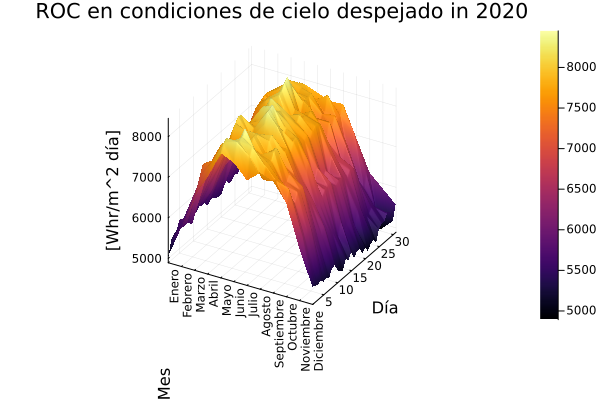
\includegraphics[
						width=\linewidth,
						height = 60mm,
						keepaspectratio
					]{Resultados/DataAnalysis/CLRSKY_SFC_SW_DWN_surface_2020_3d.png}
					\caption{Irradiación de onda corta total recibida por día en condiciones de cielo despejado durante el 2020 sobre el lugar seleccionado}
					\label{fig:CLRSKY_SFC_SW_DWN_surface_2020_3d}
				\end{subfigure}
				\hfill
				\begin{subfigure}[t]{0.45\linewidth}
					\centering
					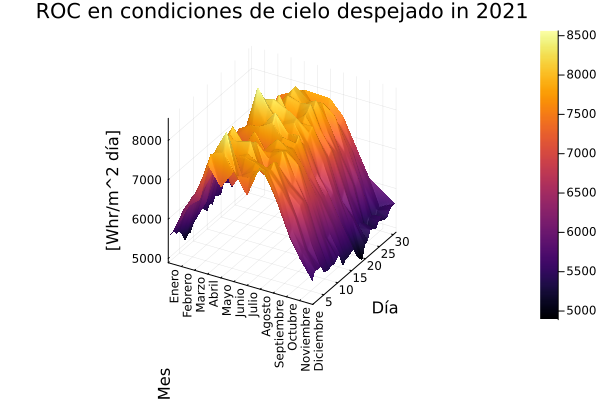
\includegraphics[
						width=\linewidth,
						height = 60mm,
						keepaspectratio
					]{Resultados/DataAnalysis/CLRSKY_SFC_SW_DWN_surface_2021_3d.png}
					\caption{Irradiación de onda corta total recibida por día en condiciones de cielo despejado durante el 2021 sobre el lugar seleccionado}
					\label{fig:CLRSKY_SFC_SW_DWN_surface_2021_3d}
				\end{subfigure}
			\end{figure}
			
			\begin{figure}[H]\ContinuedFloat
				\begin{subfigure}[t]{0.45\linewidth}
					\centering
					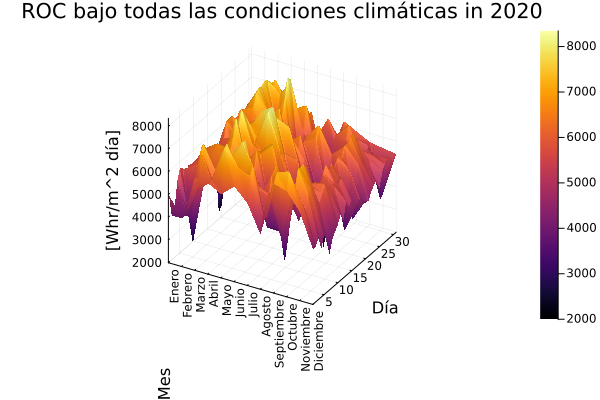
\includegraphics[
						width=\linewidth,
						height = 60mm,
						keepaspectratio
					]{Resultados/DataAnalysis/ALLSKY_SFC_SW_DWN_surface_2020_3d.png}
					\caption{Irradiación de onda corta total recibida por día bajo todas las condiciones climáticas durante el 2020 sobre el lugar seleccionado}
					\label{fig:ALLSKY_SFC_SW_DWN_surface_2020_3d}
				\end{subfigure}
				\hfill
				\begin{subfigure}[t]{0.45\linewidth}
					\centering
					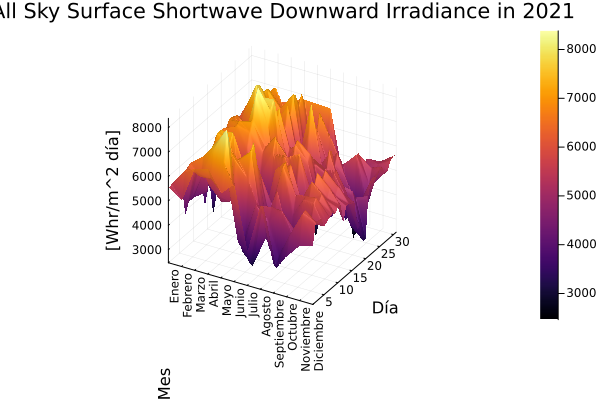
\includegraphics[
						width=\linewidth,
						height = 60mm,
						keepaspectratio
					]{Resultados/DataAnalysis/ALLSKY_SFC_SW_DWN_surface_2021_3d.png}
					\caption{Irradiación de onda corta total recibida por día bajo todas las condiciones climáticas durante el 2021 sobre el lugar seleccionado}
					\label{fig:ALLSKY_SFC_SW_DWN_surface_2021_3d}
				\end{subfigure}
			\end{figure}
			
			\begin{figure}[H]\ContinuedFloat
				\begin{subfigure}[t]{0.45\linewidth}
					\centering
					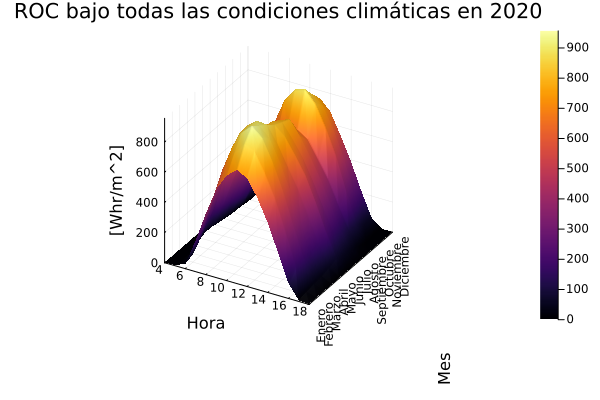
\includegraphics[
						width=\linewidth,
						height = 60mm,
						keepaspectratio
					]{Resultados/DataAnalysis/ALLSKY_SFC_SW_DWN_3d_mean_2020.png}
					\caption{Irradiación de onda corta promedio recibida por hora bajo todas las condiciones climáticas durante el 2020 sobre el lugar seleccionado}
					\label{fig:ALLSKY_SFC_SW_DWN_3d_mean_2020}
				\end{subfigure}
				\hfill
				\begin{subfigure}[t]{0.45\linewidth}
					\centering
					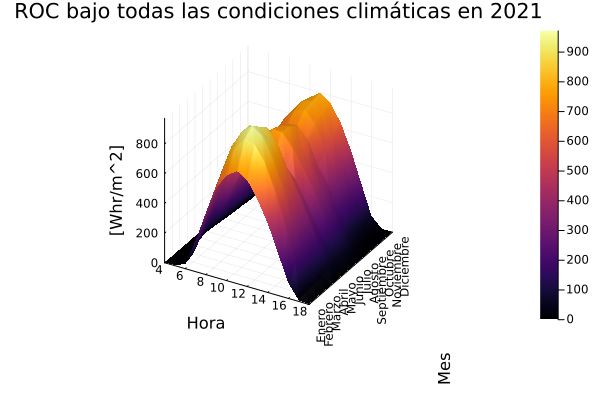
\includegraphics[
						width=\linewidth,
						height = 60mm,
						keepaspectratio
					]{Resultados/DataAnalysis/ALLSKY_SFC_SW_DWN_3d_mean_2021.png}
					\caption{Irradiación de onda corta promedio recibida por hora bajo todas las condiciones climáticas durante el 2021 sobre el lugar seleccionado}
					\label{fig:ALLSKY_SFC_SW_DWN_3d_mean_2021}
				\end{subfigure}
				\caption{Irradiación de onda corta recibida en el lugar físico de experimentación durante 2020 y 2021}
				\label{fig:SFC_SW_DWN}
			\end{figure}

		\subsection{Temperatura}
			
			\begin{figure}[H]
				\centering
				\begin{subfigure}[t]{\linewidth}
					\centering
					\includegraphics[
						width=\linewidth,
						height=70mm,
						keepaspectratio
					]{Resultados/DataAnalysis/Temperatura-promedio-por-hora-en-Ciudad-de-México.png}
					\\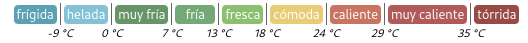
\includegraphics[
						width=0.8\linewidth,
						keepaspectratio
					]{Resultados/DataAnalysis/WeatherSpark-Temperatura-Leyenda.png}
					\caption{Temperatura promedio por hora en Ciudad de México}
					\label{fig:Temperatura-promedio-por-hora-en-Ciudad-de-México}
				\end{subfigure}
			\end{figure}
			\begin{figure}\ContinuedFloat
				\begin{subfigure}[t]{\linewidth}
					\centering
					\includegraphics[
						width=\linewidth,
						height=70mm,
						keepaspectratio
					]{Resultados/DataAnalysis/Temperatura-por-hora-en-2022-Ciudad-de-México.png}\\
					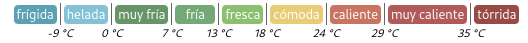
\includegraphics[
						width=0.8\linewidth,
						keepaspectratio
					]{Resultados/DataAnalysis/WeatherSpark-Temperatura-Leyenda.png}
					\caption{Temperatura por hora del 2022 en la Ciudad de México}
					\label{fig:Temperatura-por-hora-en-2022-Ciudad-de-México}
				\end{subfigure}
				\caption{Mapas de temperaturas de la Ciudad de México}
				\floatfoot{Los gráficos fueron obtenidos de \href{https://es.weatherspark.com/y/5674/Clima-promedio-en-Ciudad-de-México-México-durante-todo-el-año}{\textcopyright WeatherSpark.com}}
				\label{fig:Temperatura-CDMX}
			\end{figure}
			
		\section{Magnitud del perfil de velocidad del viento}
			
			\begin{figure}[H]
				\centering
				\begin{subfigure}[t]{0.45\linewidth}
					\centering
					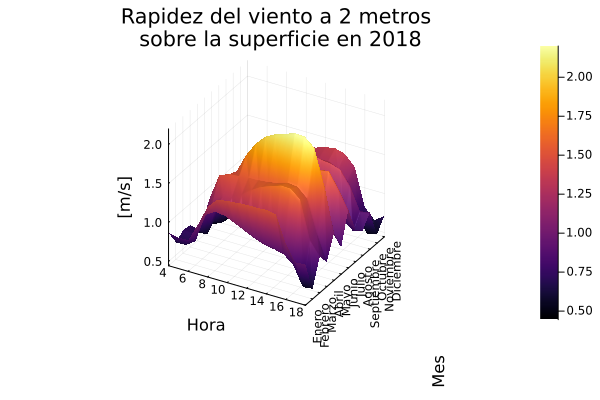
\includegraphics[
						width=\linewidth,
						height = 60mm,
						keepaspectratio
					]{Resultados/DataAnalysis/WS2M_3d_mean_2018.png}
					\caption{Rapidez promedio por hora del viento durante 2018 sobre el lugar seleccionado}
					\label{fig:WS2M_3d_mean_2018}
				\end{subfigure}
				\hfill
				\begin{subfigure}[t]{0.45\linewidth}
					\centering
					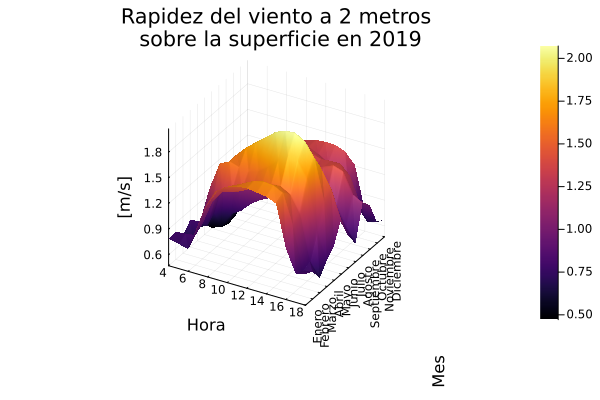
\includegraphics[
						width=\linewidth,
						height = 60mm,
						keepaspectratio
					]{Resultados/DataAnalysis/WS2M_3d_mean_2019.png}
					\caption{Rapidez promedio por hora del viento durante 2019 sobre el lugar seleccionado}
					\label{fig:WS2M_3d_mean_2019}
				\end{subfigure}
			\end{figure}
			
			\begin{figure}[H]\ContinuedFloat
				\begin{subfigure}[t]{0.45\linewidth}
					\centering
					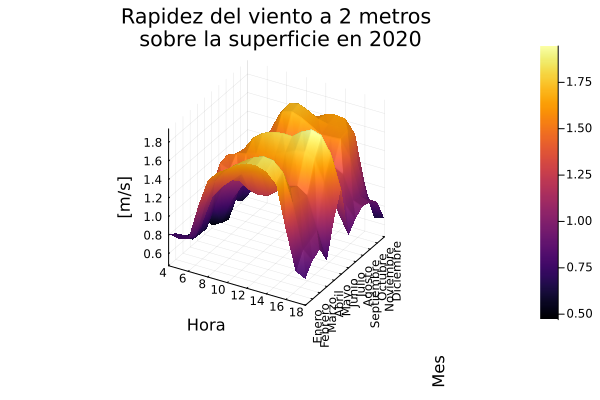
\includegraphics[
						width=\linewidth,
						height = 60mm,
						keepaspectratio
					]{Resultados/DataAnalysis/WS2M_3d_mean_2020.png}
					\caption{Rapidez promedio por hora del viento durante 2020 sobre el lugar seleccionado}
					\label{fig:WS2M_3d_mean_2020}
				\end{subfigure}
				\hfill
				\begin{subfigure}[t]{0.45\linewidth}
					\centering
					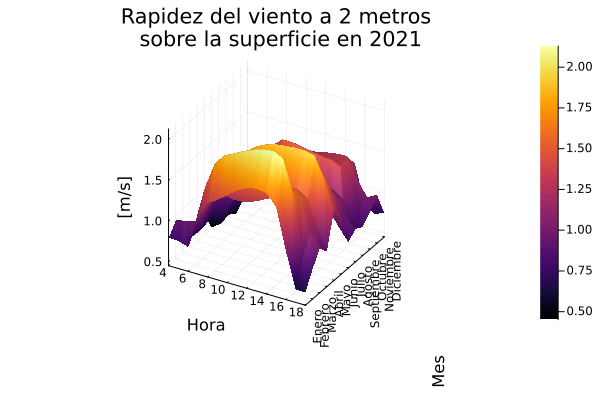
\includegraphics[
						width=\linewidth,
						height = 60mm,
						keepaspectratio
					]{Resultados/DataAnalysis/WS2M_3d_mean_2021.png}
					\caption{Rapidez promedio del viento durante 2021 sobre el lugar seleccionado}
					\label{fig:WS2M_3d_mean_2021}
				\end{subfigure}
				\caption{Rapidez promedio por hora del viento sobre el lugar seleccionado}
				\label{fig:WS2M_3d_mean}
			\end{figure}